\chapter{Design and Implementation}

The following chapter goes through the most important design considerations and their implementation.
Where appropriate, it includes a comparison to Existing Software.
Following a top-down approach, it starts with the overall architecture and the build and deployment process, continues with \gls{ui} and branding/communication aspects, and ends with a description of efficiency, device support, security, accessibility, and learning content details.
The source code is hosted at Github\footnote{Up-to-date state: \url{https://github.com/durasj/chipsandcode/}. At the time of writing: \url{https://github.com/durasj/chipsandcode/tree/6decf0}.} - referred to as Repository from now on.

\section{Overall Architecture}

As can be seen in Figure~\ref{fig:design-architecture}, Proposed Software is primarily a client-side web application.
This decision was made for two reasons:

\begin{itemize}
    \item \textbf{Connectivity}: To make sure the application does not depend on an internet connection and is available with poor or even no connectivity. This also means the design should not be disadvantaged in this regard compared to a desktop application.
    \item \textbf{Reproducibility}: No dependence on the cloud means it should be much easier to deploy to any (free) CDN, any simple web hosting, or even run locally or bundled as an Electron\footnote{Available at \url{https://www.electronjs.org}.} - desktop - or a Capacitor\footnote{Available at \url{https://capacitorjs.com/}.} - mobile - application.
\end{itemize}

To double down on this approach, it is also a \gls{pwa}, which means it can be installed on any combination of a major internet browser and \gls{os}.
Thanks to a service worker\footnote{See \url{https://developer.mozilla.org/en-US/docs/Web/API/Service_Worker_API}.} that is configured to cache all assets as soon as the user visits the website, all functionality should be available at any point, even once the user loses the connection.

\begin{figure}[H]
    \centering
    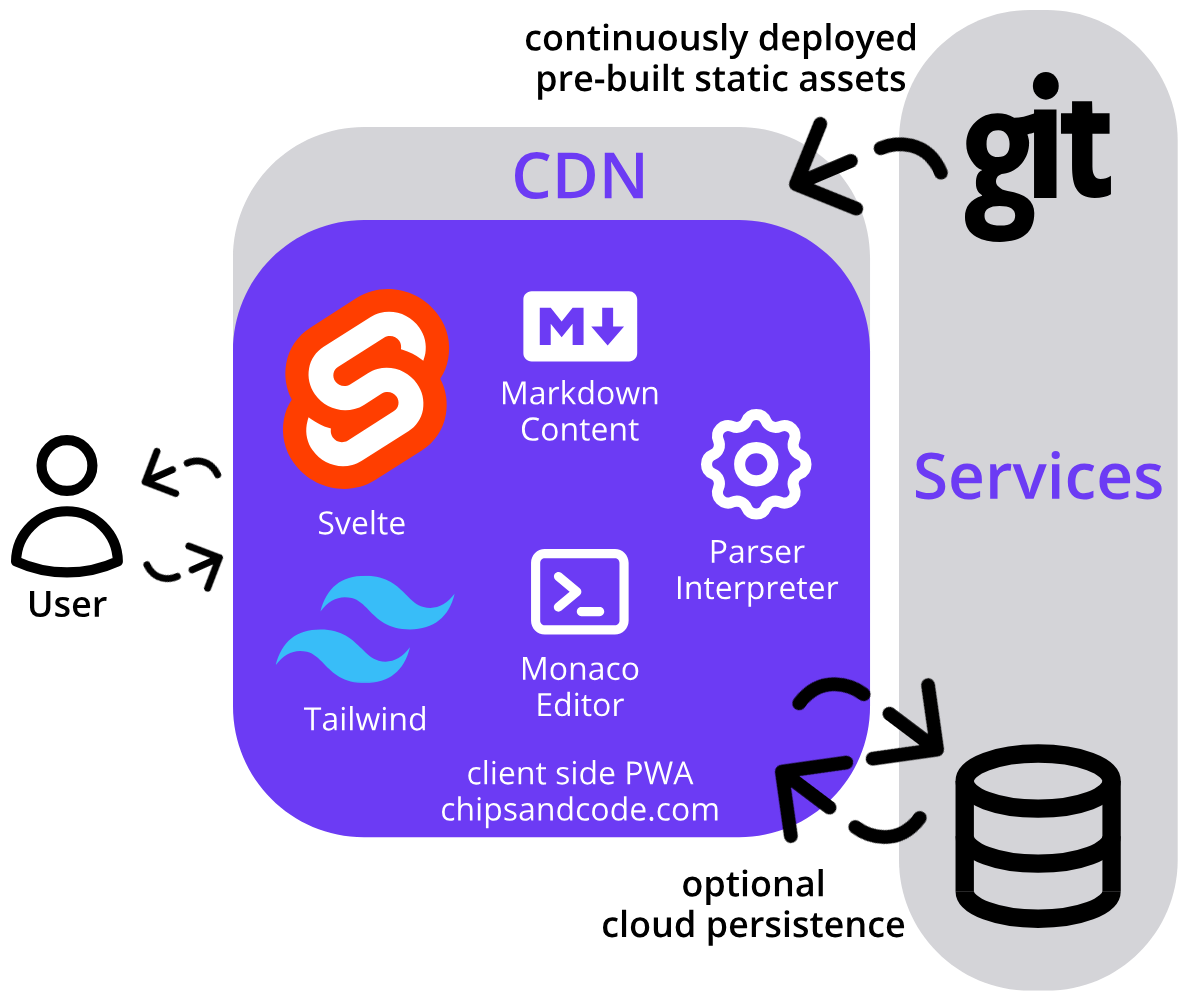
\includegraphics[width=300pt, keepaspectratio]{Architecture}
    \caption{High-level architecture diagram.}
    \label{fig:design-architecture}
\end{figure}

\section{Build and Deployment}

To enable the static file approach, the whole application has to be built ahead of time during the building phase instead of relying on \gls{ssr}.
Although Sveltekit\footnote{Available at \url{https://kit.svelte.dev}.} used for this project defaults to platform-specific \gls{ssr}\footnote{See \url{https://kit.svelte.dev/docs/adapters}}, it is possible to configure it to generate static assets and work as a \gls{spa} for pages that are not completely static\footnote{See \url{https://kit.svelte.dev/docs/adapter-static} and \url{https://kit.svelte.dev/docs/single-page-apps}.}.
In this case, the resulting bundle of static files is deployed via Cloudflare Pages\footnote{See \url{https://pages.cloudflare.com/}.}, but there are many equivalent services that can easily host static assets for free.
For a proper \gls{cd} implementation, the build is triggered on push to Repository and every branch is deployed as $branch.chipsandcode.pages.dev$.
The $main$ branch is mapped to the primary domain name \href{https://chipsandcode.com/}{chipsandcode.com}.

Optionally, it is possible to persist files to the cloud - in this case, a simple custom-made \gls{rest} \gls{api} written as a serverless application running on Cloudflare Workers\footnote{See \url{https://workers.cloudflare.com}.}.
The \gls{api} is consciously kept separately from the client-side application, although it does re-use code where it makes sense, e.g. validation schemas.

The same branch-level deployment applies to the server-side code.
However, one limitation is the storage is not separated for each branch.
Rather, there are only two key-value namespaces\footnote{Using Cloudflare KV, see \url{https://www.cloudflare.com/developer-platform/workers-kv}.} for production and development, with the latter used for branch previews as well.
Even though the cloud functionality is optional, it was still kept to a minimum (it is only about 200 lines of code) so that it is easily replaceable.
Additionally, local development does not depend on Cloudflare as it uses a simulated local environment with a SQLite database\footnote{Using Miniflare, see \url{https://github.com/cloudflare/miniflare}.}.

All in all, while Cloudflare deployment is mentioned in the supplied README, anybody who wants to contribute or adapt the project does not need to worry about it if they do not want to.
The cloud functionality is opt-in even for developers and can be enabled by setting a single $.env$ variable.

\section{User Interface}

This section covers key \gls{ui} aspects.
It always starts with design decisions from the user's perspective before moving on to an explanation of how technology enabled that.

\subsection{Interactions}

In line with the premise the time and difficulty of using a learning tool is important (see \autoref{sec:software-design}), Proposed Software minimises the friction when the user transitions from learning content to learning tool and shortens the cycle of "trial and error".
Figure~\ref{fig:design-hdl-steps} shows a comparison between Existing Software (left) and Proposed Software (right)\footnote{See video for context: \url{https://youtu.be/mnSuqmvn4hg}.} in terms of steps needed to iterate on an assignment to implement the chip's \gls{hdl}.
As we can see, with Proposed Software, the flow is linear and with only simple steps like "scroll down" that are natural.
This is in contrast to Existing Software, which has a higher number of steps that can introduce opportunities for confusion and mistakes.
Some of the simplification comes from the web, as the learning tool can be easily embedded within the content.
On top of that, there are two other relevant features:

\begin{itemize}
    \item \textbf{Code Editor Integration}: The tool has a built-in code editor so that the learner does not have to switch context. Specifically, it integrates Monaco Editor\footnote{Available at \url{https://microsoft.github.io/monaco-editor/}.}, which is the same library underneath the most popular \gls{ide} (see \autoref{sec:text-code}). It is additionally configured with custom themes and languages to fit within the content and provide syntax highlighting\footnote{See \url{https://github.com/durasj/chipsandcode/blob/6decf0/src/lib/editor/index.ts}.}. Moreover, one more feature that is integrated right into the tool is a visual diff of the output. As can be seen in Figure~\ref{fig:design-diff}, while Existing Software requires the learner to leave the \gls{ui} and use a \gls{cli} utility with a confusing output, Proposed Software provides a clear indication of all rows and even individual values that are wrong.
    \item \textbf{Automatisation}: If there is no benefit in having the user perform a manual action, the interface reacts in real-time to lower friction. In this case, it means on any change in \gls{hdl}, \gls{tst}, output, or values of input pins, the interface recalculates the outputs. Also, all output comparisons are evaluated at once so that the user has more information to base their decision on.
\end{itemize}

\begin{figure}[H]
    \centering
    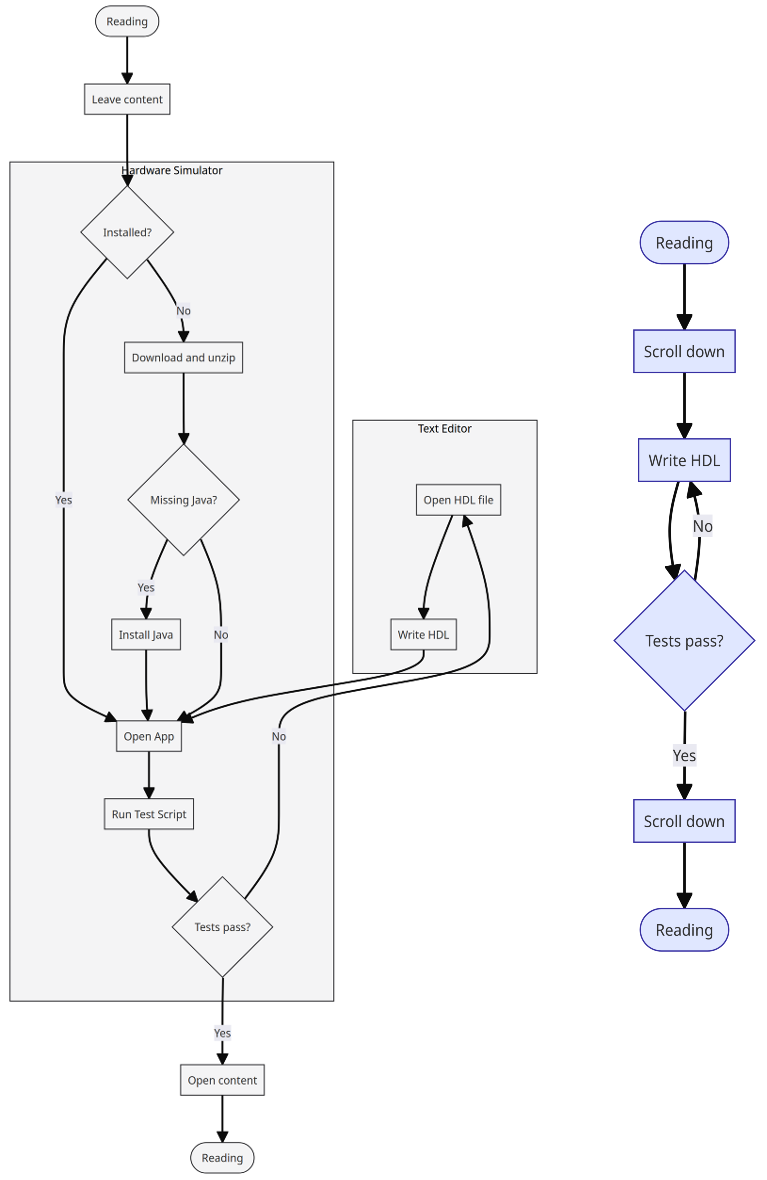
\includegraphics[width=360pt, keepaspectratio]{Flow_HDL_Comparison}
    \caption{Comparison of steps needed to iterate on an \gls{hdl} assignment.}
    \label{fig:design-hdl-steps}
\end{figure}

\begin{figure}[H]
    \centering
    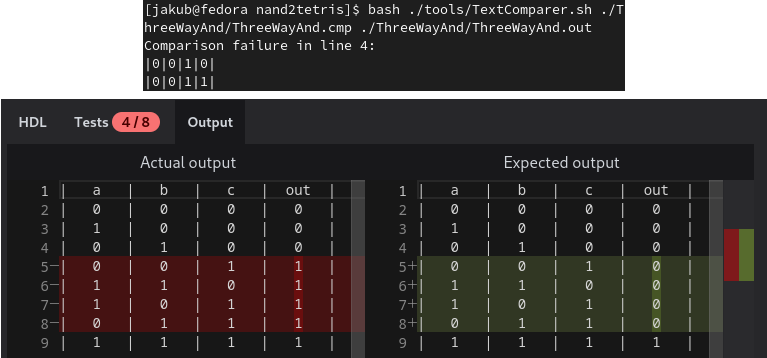
\includegraphics[width=300pt, keepaspectratio]{Output_Diff}
    \caption{Existing Software's Text Comparer (top) and Proposed Software's visual output diff (bottom).}
    \label{fig:design-diff}
\end{figure}

\subsection{Error Handling}

Since it is assumed user errors are likely, especially when introducing new concepts, with Proposed Software, the intention is to prevent user errors when it is possible and try to make them helpful when not.
This is achieved by combining:

\begin{itemize}
    \item \textbf{Robust Parser}: Some syntax errors (e.g. due to extra white space) are prevented, while other are streamlined using real-time inline errors with feedback suggesting expected token, as can be seen in Figure~\ref{fig:design-syntax-errors}. While Existing Software uses procedural code for parsing, Proposed Software utilises Regular Expression-based lexer generator\footnote{Moo, available at: \url{https://github.com/no-context/moo}.} and an Earley parser generator\footnote{Nearley, available at: \url{https://github.com/no-context/moo}.}. Instead of using hundreds of lines of procedural code, Proposed Software uses one file with less than a hundred lines of transparent token definition, grammar, and post-processing code - see Appendix~\ref{appendix:hdl-railroad}, \ref{appendix:hdl-grammar}, \ref{appendix:tst-railroad}, and \ref{appendix:tst-grammar}.
    \item \textbf{Simple Error Messages}: Similarly to syntax errors, other errors, like errors in logic, are simple and provide details and suggestions. Figure~\ref{fig:design-pin-error} shows Existing Software and Proposed Software are comparable, but Proposed Software offers a more focused and detailed (notice the mention of input pins) error message and especially a suggestion. As can be seen in Figure~\ref{fig:design-text-ast-graph}, Proposed Software creates a graph with pins as vertices and edges that can reference chips. Then, it is possible to traverse the graph from inputs using \gls{bfs} and determine which connections are invalid or if the implementation contains cycles.
\end{itemize}

\begin{figure}[H]
    \centering
    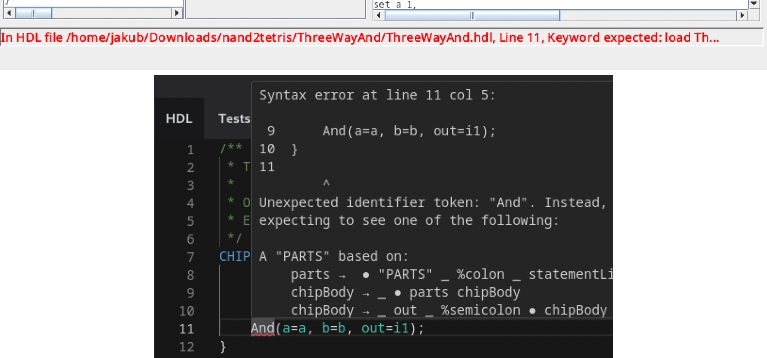
\includegraphics[width=380pt, keepaspectratio]{Syntax_Error}
    \caption{Existing Software's (top) and Proposed Software's (bottom) syntax error handling.}
    \label{fig:design-syntax-errors}
\end{figure}

\begin{figure}[H]
    \centering
    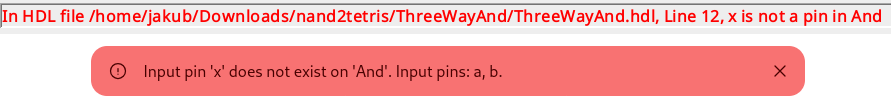
\includegraphics[width=380pt, keepaspectratio]{Pin_Error}
    \caption{Existing Software's (top) and Proposed Software's (bottom) pin connection error handling.}
    \label{fig:design-pin-error}
\end{figure}

\begin{figure}[H]
    \centering
    \includesvg[width=380pt, keepaspectratio]{Text_AST_Graph}
    \caption{\gls{hdl} processing from text to chip connection graph.}
    \label{fig:design-text-ast-graph}
\end{figure}

\section{Branding and Presentation}

In line with the advice explored in \autoref{sec:oss-essential-steps}, the project is available under the name Chips and Code at \href{chipsandcode.com}{https://chipsandcode.com}.
It makes use of a consistent brand identity - logo, colours (accessible combination of violet and orange), and fonts.
There are two different mission statements depending on the target audience:

\begin{enumerate}
    \item \textbf{Wide Audience}: "Wondering how computers work? Find out by embarking on the journey of building your own computer from scratch, from chips to code. No prerequisites - start for free from the browser."
    \item \textbf{Technical Audience}: "Chips and Code – reimagined Nand2Tetris tools powered by the modern web with better User Experience."
\end{enumerate}

Both \href{chipsandcode.com}{https://chipsandcode.com} and Repository mention the project is in a "preview" or "work in progress" state.
Repository also features a list of current and planned features and very simple documentation on how to get started with the development and how to deploy.
Moreover, Repository contains an animated demo of the software.
Features and bugs are managed in Repository that also offers a simple discussion forum\footnote{See \url{https://github.com/durasj/chipsandcode/discussions}.} prepared for communication.
Basic information and links are also available on the website's About page\footnote{See \url{https://chipsandcode.com/about}}.

\section{Efficiency}

One of the aims was to keep the application as small and efficient as possible.
This brings benefits not only for less equipped users (e.g. from developing countries) with lower power devices and limited network connection but also for users with powerful client devices and fast internet connection for whom the application loads and responds instantly.
There are several technologies that enabled this:

\begin{itemize}
    \item \textbf{Svelte and Tailwind}: Although each has a different responsibility - the former is a front-end framework\footnote{Available at: \url{https://svelte.dev}.} and the latter a \gls{css} framework\footnote{Available at: \url{https://tailwindcss.com}}, both share the same philosophy - no overhead of the library. Svelte achieves this by generating tailor-mode optimised code during the build instead of using a run-time rendering library. Tailwind, on the other hand, uses atomic styles, of which only a small subset is often reused throughout the app, and the rest is removed during the build.
    \item \textbf{Three Shaking, Chunking, Prerendering}: All imports are automatically analysed by Vite\footnote{See \url{https://vitejs.dev/guide/features.html}.}, unused parts of the code are removed (three shaking), and the rest is split into chunks for faster initial loads so that larger features like Monaco Editor do not block the initial load. Prerendering done at build time also speeds up the initial load as the page loads instantly as a simple \gls{html} and then is hydrated via \gls{js}.
    \item \textbf{Small Assets}: Any hard-earned efficiency gains could be easily ruined with unoptimised multimedia assets like images. Therefore, whenever possible, Proposed Software uses vector graphics (SVGs), and when not, modern efficient AVIF or WEBP image formats with JPEF fallback using the picture element\footnote{See \url{https://developer.mozilla.org/en-US/docs/Web/HTML/Element/picture}.}. This is done automatically and includes resizing and low-quality variants used for the initial load\footnote{Using $svelte-img$, available at: \url{https://github.com/zerodevx/svelte-img}.}. Proposed Software also does not use custom fonts but instead relies on a system font stack\footnote{See \url{https://bitsofco.de/the-new-system-font-stack/}.}.
    \item \textbf{Preload}: Apart from the pre-caching done using the previously mentioned service worker, all crucial modules are marked for preload\footnote{See \url{https://developer.mozilla.org/en-US/docs/Web/HTML/Attributes/rel/modulepreload}.} so that the browser can process them ahead of time in parallel. Additionally, anytime the user hovers or starts a touch gesture on an internal link, it is preloaded with high priority in a split second before the tap/click actually happens\footnote{See \url{https://kit.svelte.dev/docs/link-options}.}.
\end{itemize}

The result of these optimisations can be not only observed subjectively but also, to some extent, captured in the size of the page or the whole application and using performance tests.
Figure~\ref{fig:design-size-comparison} features a chart showing the size of Proposed Software compared to Existing Software.
Keep in mind that Proposed Software includes learning content, a code editor with syntax highlighting, and does not require any additional third-party runtime like a \gls{jvm}.

While the zip file with Existing Software is 700 kB, we can also consider the size of the website (1.7 MB\footnote{Transferred over the network. Assuming we land directly on \url{https://www.nand2tetris.org/software}.}) and of the Google Drive link (700 kB\footnote{Transferred over the network. When visiting linked \url{https://drive.google.com/file/d/1xZzcMIUETv3u3sdpM_oTJSTetpVee3KZ/view} without a Google account.}) we likely have to visit to download it.
In case the user has to download Java SE to run Existing Software, it adds from 62 MB on Windows to 93 MB on Linux.
If we assume a poor internet connection with 1 Mb/s download speed, both Existing Software and Proposed Software can be downloaded within 30 seconds.
Java SE 8, on the other hand, would take up to 12 minutes.
However, in terms of size, to put it into perspective, even within developing countries, 100 MB of data costs at most 1\% of average monthly income \parencite{Rodriguez_2022}.

Although the actual size of Proposed Software is about 5 MB (most of which is Monaco Editor), only about 1.5 MB is actually transferred over the network\footnote{When using Brotli supported by over 95\% web clients globally, see \url{https://caniuse.com/brotli}.}.
That being said, since Proposed Software does not yet contain all of the expected learning material and functionality, we can assume the final size to be 2 MB.
That is comparable to an average website \parencite{Indigo_2022} - a single page of a website, not a whole \gls{pwa} with a code editor, etc.
Lighthouse performance report shown in Figure~\ref{fig:design-lighthouse-performance} captures a score of 100/100 for the most complex page with long learning content and embedded Hardware \gls{ide}.

\begin{figure}[H]
    \centering
    \includesvg[width=360pt, keepaspectratio]{Plot_Size_Comparison}
    \caption{Size comparison between Proposed Software and Existing Softare.}
    \label{fig:design-size-comparison}
\end{figure}

\begin{figure}[H]
    \centering
    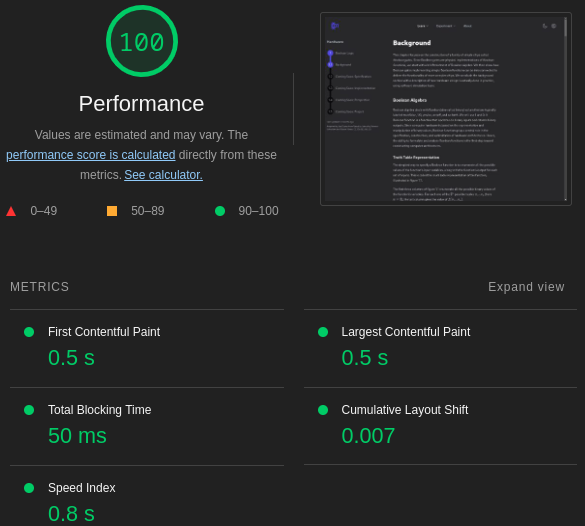
\includegraphics[width=380pt, keepaspectratio]{Lighthouse_Performance}
    \caption{Lighthouse performance report for Proposed Software.}
    \label{fig:design-lighthouse-performance}
\end{figure}

As far as the parser goes, despite the fact it uses the Earley algorithm with a heavy use of right recursion and even considers white space during parsing (as opposed to disregarding it during lexing), it still takes within 1 ms per parse.
This was measured\footnote{Using the high-precision Performance API, see \url{https://developer.mozilla.org/en-US/docs/Web/API/Performance/measure}.} on Appendix~\ref{appendix:hdl-example} - a medium complexity (in a learning context) example with \gls{ast} output of 3 kB (JSON).
The time varied between 0.09 ms on a high-end desktop with i7 13700 and 0.78 ms on an older midrange smartphone with Snapdragon 662.

\section{Security}

Even though security was not the highest priority for Proposed Software, it still implemented essential security measures.
Deployment-level features include DNSSEC, HTTPS, or mandatory GPG-signed commits that prevent automated deployment of spoofed commits from the main branch.
As for Denial of Service attacks, Proposed Software relies primarily on Cloudflare Pages that offer unlimited free bandwidth and requests.
As far as the optional cloud functionality goes, in the worst-case scenario, it would stop working for the day after reaching 100k requests.

Only anonymous sessions were implemented, which means risks related to sensitive data were minimal.
To mitigate session fixation, sessions were using $HttpOnly$ and $Secure$ cookies.
Parsers and interpreters were not using $eval$ or similar techniques that would allow the execution of arbitrary code.

\section{Accessibility}

Proposed Software was built from the beginning to be accessible to the widest range of users, and this was reflected during the design, implementation, and testing.
During the design and implementation, that meant focusing on the simplicity of the \gls{ui}, paying attention to proper use of semantics, use of \gls{aria} \glspl{api} if necessary, and continuous use of automated checks\footnote{Using svelte-check, available at: \url{https://www.npmjs.com/package/svelte-check}.} and semi-automated tools like aXe DevTools\footnote{Available at: \url{https://chrome.google.com/webstore/detail/axe-devtools-web-accessib/lhdoppojpmngadmnindnejefpokejbdd}.}.

\begin{figure}[H]
    \centering
    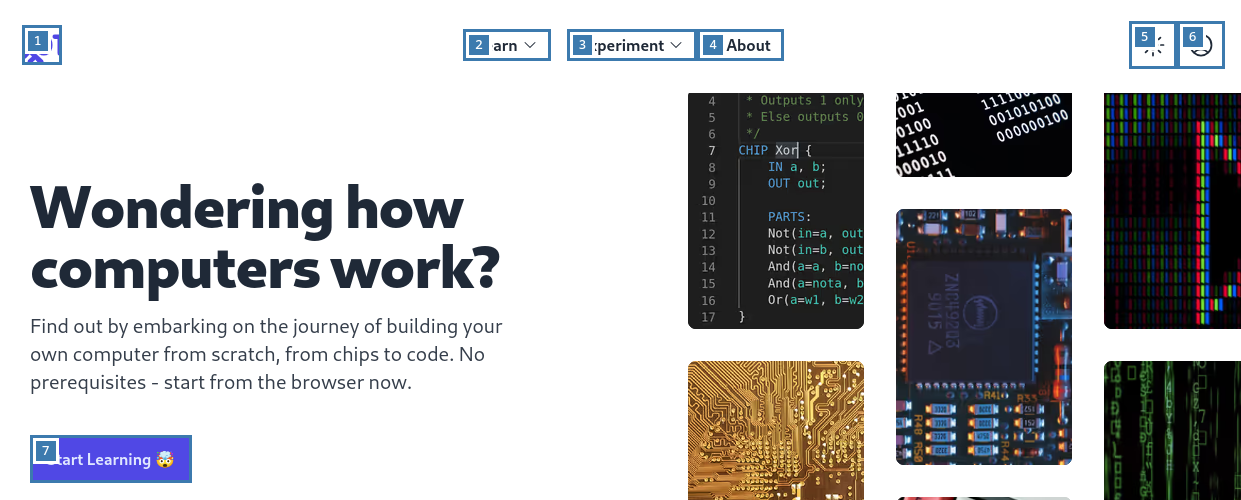
\includegraphics[width=380pt, keepaspectratio]{Axe_Focus_Order}
    \caption{Example use of aXe DevTools to verify focus order.}
    \label{fig:design-axe-focus}
\end{figure}

All accessibility-related features of Monaco Editor\footnote{See \url{https://github.com/microsoft/monaco-editor/wiki/Monaco-Editor-Accessibility-Guide}.} were bundled, and the editor should be reasonably accessible despite its complexity.
Similarly, despite the fact Proposed Software uses client-side routing, navigation triggers an announcement of new pages and handles the focus\footnote{See \url{https://kit.svelte.dev/docs/accessibility}.}.
Proposed Software also contains an accessibility statement, which, among else, prompts users to make use of the accessibility tools built into the browser.
During the automated testing, the used approach follows the premise the \gls{ui} must be easy to target and control using the same semantics utilised by accessibility tools.
For example, all elements are findable using their text content or labels\footnote{Using Testing Library packages, see \url{https://testing-library.com/docs}.} instead of using "technical" selectors like identifiers or identifiers dedicated to automated tests only.

\section{Device Support}

Designing for a wide range of users means also designing for a wide range of client devices.
Thanks to the design decision to implement Proposed Software as a client-side web application, it can be run on a rather wide range of devices by default, even without any optimisations.
To make the use from these different devices comfortable, during the development, all pages were tested they work properly on a realistic range of screen widths by slowly scaling the width from 400px (or equivalent) to 1920px (or equivalent).
Figure~\ref{fig:design-screenshot-ide-mobile} shows an example of the Hardware \gls{ide} page on a smartphone.

\begin{figure}[H]
    \centering
    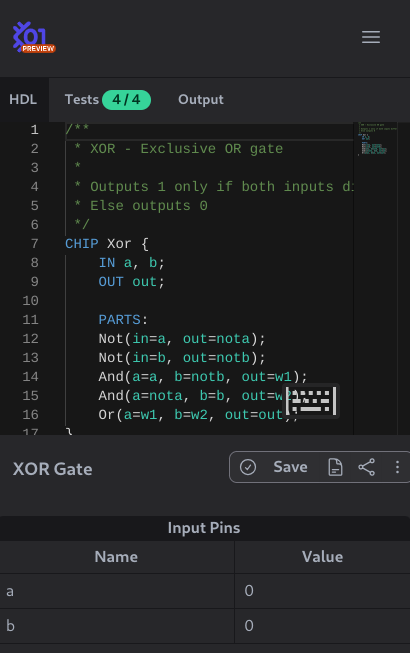
\includegraphics[width=240pt, keepaspectratio]{Screenshot_IDE_Mobile}
    \caption{Hardware \gls{ide} viewed from a smarrtphone.}
    \label{fig:design-screenshot-ide-mobile}
\end{figure}

The high market share of modern web browsers and the \gls{ui} responsivity mean Proposed Software should be usable by the vast majority of internet users - excluding only users of unsupported browsers like Internet Explorer that now account for $<1\%$\footnote{See \url{https://gs.statcounter.com}.}.
Compared to that, based on the statistics gathered in \autoref{sec:device-types}, Existing Software would be globally accessible only from 44\% of devices used to browse the web.
However, if we consider only users that rely on smartphones, within developing countries, this means one-fourth of the population is unable to access Existing Software.

\begin{figure}[H]
    \centering
    \includesvg[width=380pt, keepaspectratio]{Plot_Device_Support}
    \caption{Probable percentage of supported devices.}
    \label{fig:design-device-support}
\end{figure}

\section{Learning Content}

Proposed Software includes a way to produce learning content.
This is done simply using version-controlled Markdown files that can be seen in Repository\footnote{See \url{https://github.com/durasj/chipsandcode/tree/6decf0/src/routes/learn/hardware/boolean-logic} for examples.}.
Based on the review done in \autoref{sec:text-code}, Markdown documents should be easier to write while still preserving the advantages of the plaintext input format.
Since Markdown does not allow for any custom styling, all of the content is presented consistently and can be used long-term in different forms.
Moreover, the Markdown content implementation still allows for powerful additions, namely:

\begin{itemize}
    \item \textbf{Math Expressions}: Proposed Software supports the use of TeX-like inline mathematical notation.
    \item \textbf{Embeds}: Videos or developed tools like the Hardware \gls{ide} can be easily embedded.
\end{itemize}

From the technical point of view, this is made possible thanks to Markdoc\footnote{Available at: \url{https://markdoc.dev}.}, which is used in a custom Vite plugin that parses and transforms Markdown documents to a renderable tree usable with Svelte.
Math support is made possible thanks to KaTeX\footnote{Available at: \url{https://katex.org}.}, which uses MathML and custom fonts with \gls{css} to render processed input.
Embeds, specifically, are supported via custom tags - an extension to the Markdown syntax\footnote{See \url{https://markdoc.dev/docs/tags}.}.
These features can be seen in Markdwon example in Figure~\ref{fig:design-markdown-example}.

\begin{figure}[H]
\begin{minted}[breaklines=true, fontsize=\small]{markdown}
## Example: Building a Nand Gate

One way to define a _Not_ And is `Nand(a, b) = Not(And(a, b))`.
Just some random math expression: $f(x, y)$.
And an embed for a good measure:


\end{minted}



    \caption{Example of learning content written in Markdown.}
    \label{fig:design-markdown-example}
\end{figure}
